\subsection{Desarrollo manual de un caso de soporte y extensión a otros casos}
\label{sec:caso_manual_revision}

\subsubsection{Caso de referencia y datos de entrada}

Se desarrolla el caso nominal centrado del bastidor con tres apoyos sectoriales. Se conserva la carga externa del modelo estructural de referencia, $W_r=29844$ N, para que la comparación utilice las mismas acciones. El peso calculado a partir de la masa de catálogo es
\begin{equation}
W_{\mathrm{cat}}=3032(9{,}81)=29743{,}92\ \mathrm{N}.
\label{eq:manual_peso_catalogo}
\end{equation}
La diferencia de 100,08 N entre ambas bases de carga se documenta sin modificar la corrida. El cálculo nominal que sigue utiliza 29844 N; la alternativa basada en la masa de catálogo es otra base de carga.

El rodamiento se idealiza como un cuerpo apoyado en tres puntos no colineales. Las fuerzas transmitidas por los apoyos son verticales y no se introduce una acción horizontal en este caso. La mesa se apoya en cuatro ruedas. Para el bastidor se conserva la idealización lineal de la corrida, con su peso propio de barras de 1648,74 N, obtenido del caso de peso propio de la exportación original.

La Figura~\ref{fig:planta_manual_revision} distingue los apoyos sectoriales de las ruedas. El origen de la planta coincide con el centro nominal del rodamiento; $X$ es transversal a los rieles y $Y$ sigue su dirección. Las coordenadas se utilizan para establecer brazos de momento, mientras que las cotas describen la geometría de forma directa. El plano $Z=0$ de esta figura es el plano analítico de las barras; no representa la cota del piso del taller.

\begin{figure}[htbp]
\centering
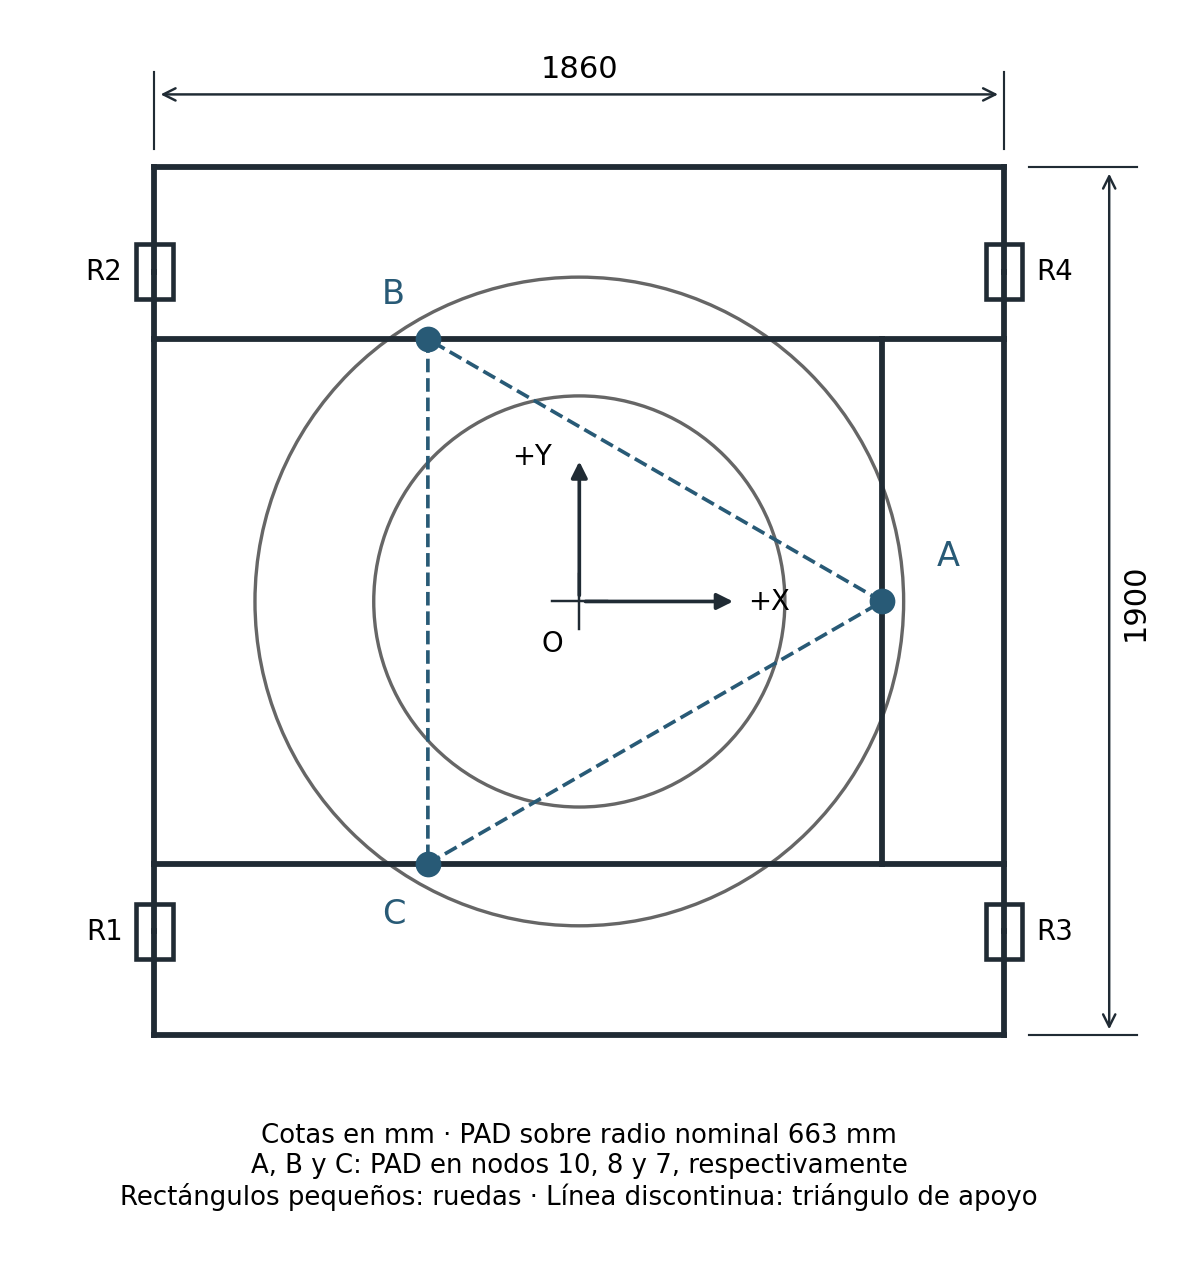
\includegraphics[width=0.92\textwidth]{images/planta_caso_manual}
\caption{Planta de cálculo reconstruida a partir de las coordenadas y la conectividad de la hoja exportada de SAP2000. El rodamiento está centrado; las barras se representan por sus líneas medias. Elaboración propia.}
\label{fig:planta_manual_revision}
\end{figure}

La Tabla~\ref{tab:coordenadas_manual_revision} recoge las coordenadas empleadas en el caso manual.

\begin{table}[htbp]
\centering\small\singlespacing
\caption{Posiciones utilizadas en el cálculo nominal}
\label{tab:coordenadas_manual_revision}
\begin{tabular}{lrrl}
\toprule
\textbf{Elemento} & \textbf{$X$ (mm)} & \textbf{$Y$ (mm)} & \textbf{Nodo SAP}\\
\midrule
Apoyo A & 663,00 & 0,00 & 10\\
Apoyo B & $-331,50$ & 574,18 & 8\\
Apoyo C & $-331,50$ & $-574,18$ & 7\\
Rueda 1 & $-930,00$ & $-722,00$ & 2\\
Rueda 2 & $-930,00$ & 722,00 & 5\\
Rueda 3 & 930,00 & $-722,00$ & 13\\
Rueda 4 & 930,00 & 722,00 & 16\\
\bottomrule
\end{tabular}
\par\smallskip\footnotesize
Fuente: tabla de coordenadas nodales de la exportación original de SAP2000 (Anexo~\ref{anx:programas}). La ordenada 574,18 mm conserva el redondeo de esa exportación; el valor geométrico nominal es aproximadamente 574,175 mm.
\end{table}

\subsubsection{Resolución del equilibrio del rodamiento}

Se aplica el equilibrio de fuerzas y momentos con las reacciones positivas hacia arriba \cite{shigley2015}. Para una resultante vertical que pasa por $(x_r,y_r)$, las ecuaciones son
\begin{equation}
\begin{bmatrix}
1&1&1\\
663&-331{,}5&-331{,}5\\
0&574{,}18&-574{,}18
\end{bmatrix}
\begin{bmatrix}R_A\\R_B\\R_C\end{bmatrix}
=
\begin{bmatrix}W_r\\W_r x_r\\W_r y_r\end{bmatrix}.
\label{eq:manual_matriz_pad}
\end{equation}
La primera fila se expresa en N; las dos restantes, en N\,mm. Para el caso centrado se reemplazan $x_r=y_r=0$ y $W_r=29844$ N:
\begin{align}
R_A+R_B+R_C &=29844,\\
663R_A-331{,}5R_B-331{,}5R_C&=0,\\
574{,}18R_B-574{,}18R_C&=0.
\end{align}
De la tercera ecuación se obtiene $R_B=R_C$. Al sustituir esta relación en la segunda, resulta $663R_A-663R_B=0$ y, por tanto, $R_A=R_B$. Finalmente,
\begin{equation}
\boxed{R_A=R_B=R_C=9948\ \mathrm{N}=9{,}948\ \mathrm{kN}.}
\label{eq:manual_reacciones_pad}
\end{equation}

La suma de las reacciones es 29844 N y sus momentos respecto de los dos ejes se anulan. Sobre el bastidor actúan las fuerzas opuestas, dirigidas hacia abajo. Estas fuerzas coinciden con los tres valores $F_3=-9948$ N registrados en la hoja de cargas nodales. Esa hoja contiene las cargas introducidas en SAP; no es un resultado de una simulación del contacto entre el rodamiento y los apoyos.

Para extender el cálculo a una resultante excéntrica, la resolución de la misma matriz da
\begin{align}
R_A&=\frac{W_r}{3}\left(1+\frac{2x_r}{663}\right),\\
R_B&=\frac{W_r-R_A}{2}+\frac{W_r y_r}{2(574{,}18)},\\
R_C&=\frac{W_r-R_A}{2}-\frac{W_r y_r}{2(574{,}18)}.
\label{eq:manual_pad_general}
\end{align}
Estas expresiones permiten evaluar otras posiciones de la resultante con las mismas coordenadas de apoyo, sin repetir su desarrollo algebraico.

\subsubsection{Contacto compresivo y presión media}

En una interfaz sin amarre vertical se exige reacción normal no negativa. Si $g_i$ representa la separación entre superficies, las condiciones ideales son
\begin{equation}
R_i\geq0,\qquad g_i\geq0,\qquad R_i g_i=0.
\label{eq:manual_contacto}
\end{equation}
Para el caso centrado se adopta la hipótesis de tres apoyos asentados, $g_A=g_B=g_C=0$. Las tres reacciones calculadas son positivas, de modo que la hipótesis es estáticamente admisible. Esta comprobación corresponde a apoyos puntuales ideales; no determina la distribución real de presión en un revestimiento deformable.

El área geométrica de cada liner, representado por un sector entre radios de 638 y 688 mm y ángulo de $24^\circ$, resulta
\begin{equation}
A=\frac{24\pi}{360}\left(688^2-638^2\right)
=13885{,}840\ \mathrm{mm^2}.
\label{eq:manual_area}
\end{equation}
Si toda esa área participa en el contacto, la presión media del caso nominal es
\begin{equation}
\boxed{p_m=\frac{9948}{13885{,}840}=0{,}7164\ \mathrm{MPa}.}
\label{eq:manual_presion}
\end{equation}
El resultado establece una demanda media de referencia. Para comprobar el liner se necesita el área efectiva y la resistencia admisible correspondiente a su material, temperatura y duración de la carga. Si la huella efectiva disminuye, la presión media aumenta.

La factibilidad se evalúa antes de aceptar una reacción máxima. Como comprobación del procedimiento, una resultante situada en $x_r=-400$ mm y $y_r=0$ produce
\[
R_A=-2055{,}620\ \mathrm{N},\qquad
R_B=R_C=15949{,}810\ \mathrm{N}.
\]
La reacción negativa indica que esa terna no puede sostener la carga con contactos exclusivamente compresivos y se rechaza esa solución. No se sustituye el valor negativo por cero, porque así se perdería el equilibrio de momentos. Este ejemplo es una prueba matemática fuera del triángulo de apoyo, no una posición de trabajo del rodamiento (Figura~\ref{fig:contacto_manual_revision}).

En el caso nominal, la resultante permanece dentro del triángulo y las tres reacciones son compresivas. La tolerancia propuesta de colocación de 5 mm requiere además revisar la cobertura del aro sobre cada apoyo. El triángulo de apoyo y la huella real del liner representan comprobaciones geométricas diferentes.

\begin{figure}[htbp]
\centering
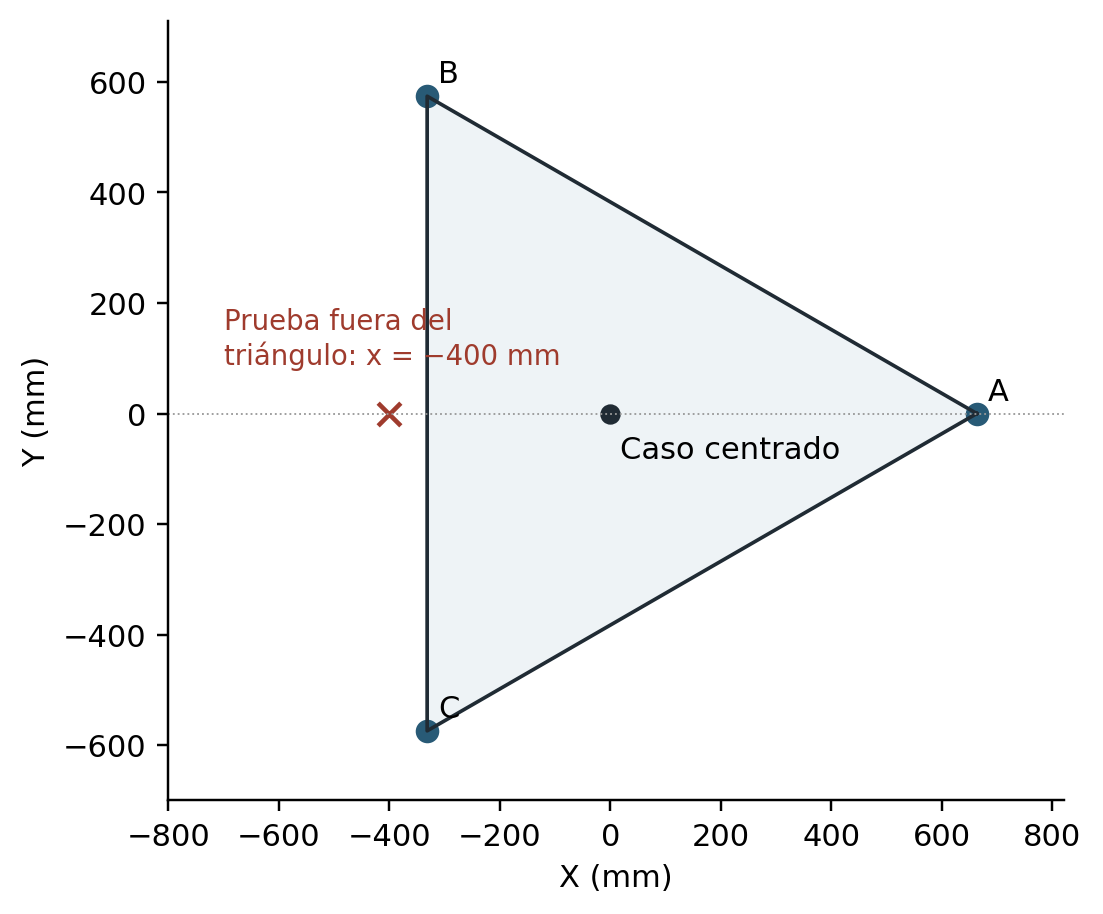
\includegraphics[width=0.84\textwidth]{images/factibilidad_pad}
\caption{Posición de la resultante del caso centrado y de la prueba matemática fuera del triángulo de apoyo. Elaboración propia a partir de las coordenadas del modelo.}
\label{fig:contacto_manual_revision}
\end{figure}

La Figura~\ref{fig:contacto_manual_revision} muestra ambas posiciones. El ejemplo exterior corresponde a una solución inadmisible porque exigiría tracción en un apoyo.

\subsubsection{Equilibrio del bastidor y reacciones en las ruedas}

La carga externa está centrada, pero la distribución de perfiles no es simétrica respecto de $X=0$: existe un miembro adicional en el lado del apoyo A. Para obtener el centro del peso propio se utilizan las longitudes y centroides de los 20 elementos de barra. Como todos tienen la misma sección y se adopta peso por unidad de longitud uniforme, el centro se calcula mediante
\begin{equation}
x_b=\frac{\sum_j L_j x_j}{\sum_j L_j},\qquad
y_b=\frac{\sum_j L_j y_j}{\sum_j L_j}.
\label{eq:manual_cg_perfiles}
\end{equation}
Con los valores de la tabla de conectividad de barras, se obtiene
\[
\sum_jL_j=12388{,}38\ \mathrm{mm},\quad
x_b=61{,}457808\ \mathrm{mm},\quad y_b\simeq0.
\]
El peso propio de barras se toma como una entrada del caso de referencia, $W_b=1648{,}74$ N. Su distribución se calcula a partir de la geometría, sin utilizar las reacciones individuales de SAP. El peso total y su primer momento respecto del plano $X=0$ son
\begin{align}
W_t&=29844+1648{,}74=31492{,}74\ \mathrm{N},\\
W_bx_b&=1648{,}74(61{,}457808)
=101327{,}946\ \mathrm{N\,mm}.
\label{eq:manual_peso_momento}
\end{align}

La geometría, las cargas y el campo vertical de la solución se consideran simétricos respecto de $Y=0$. En la idealización lineal de este caso, se conserva así la igualdad de las dos reacciones de cada lado: $R_1=R_2$ y $R_3=R_4$. Para evitar extender esta simplificación a otros escenarios, se limita a la carga vertical centrada y a los apoyos del modelo de referencia.

Al definir $R_-=R_1+R_2$ y $R_+=R_3+R_4$, el equilibrio exige
\begin{align}
R_-+R_+&=W_t,\\
930(R_+-R_-)&=W_bx_b.
\end{align}
Las reacciones individuales quedan
\begin{align}
R_1=R_2&=\frac{1}{4}\left(W_t-\frac{W_bx_b}{930}\right)
 =7845{,}9463\ \mathrm{N},\\
R_3=R_4&=\frac{1}{4}\left(W_t+\frac{W_bx_b}{930}\right)
 =7900{,}4237\ \mathrm{N}.
\label{eq:manual_ruedas}
\end{align}

La diferencia de carga entre ambos lados responde al centro del peso de los perfiles. El centro del rodamiento continúa en $(0,0)$. Tampoco debe confundirse este centro del bastidor analítico con el centro de gravedad del conjunto móvil, que incluye ruedas, mecanismos y otros accesorios. La Tabla~\ref{tab:manual_sap_revision} contrasta estas reacciones con las de la exportación de SAP2000.

\begin{table}[htbp]
\centering\small\singlespacing
\caption{Comparación de reacciones verticales del caso nominal}
\label{tab:manual_sap_revision}
\begin{tabular}{lrrr}
\toprule
\textbf{Nodo} & \textbf{Manual (N)} & \textbf{SAP (N)} & \textbf{Manual $-$ SAP (N)}\\
\midrule
2 & 7845,9463 & 7845,95 & $-0,0037$\\
5 & 7845,9463 & 7845,95 & $-0,0037$\\
13 & 7900,4237 & 7900,42 & 0,0037\\
16 & 7900,4237 & 7900,42 & 0,0037\\
\midrule
Total & 31492,7400 & 31492,74 & 0,0000\\
\bottomrule
\end{tabular}
\par\smallskip\footnotesize
Fuente: tabla de reacciones nodales de la exportación original de SAP2000, combinación nominal. El cálculo manual utiliza el peso propio total exportado y distribuye ese peso mediante la geometría de barras.
\end{table}

Las diferencias individuales son inferiores a 0,004 N, compatibles con la precisión de las tablas exportadas. El mayor error relativo es aproximadamente \SI{0.0000471}{\percent}. La comprobación confirma la suma y la distribución de reacciones del caso vertical centrado. No es una verificación independiente de la rigidez, del índice resistente ni de los contactos en situaciones de desnivel.

Las cuatro reacciones nominales son positivas. Este resultado es compatible con cuatro contactos cerrados en ese caso, pero los apoyos verticales del modelo SAP son bilaterales. La ausencia de levantamiento en otros escenarios requiere resolver las separaciones y reacciones de cada contacto; no se deduce de una sola combinación favorable.

\subsubsection{Cálculo manual de la flecha relativa a partir de SAP}

Se utiliza el travesaño comprendido entre los nodos 3 y 14, cuya luz es $L=1860$ mm. El nodo 7 está a $598{,}5$ mm del nodo 3. Para la combinación nominal, la exportación registra
\[
u_3=-0{,}117051\ \mathrm{mm},\quad
u_{14}=-0{,}117920\ \mathrm{mm},\quad
u_7=-1{,}353133\ \mathrm{mm}.
\]
La cuerda que une los extremos deformados tiene, en el nodo 7, el desplazamiento
\begin{align}
u_c&=u_3+\frac{598{,}5}{1860}(u_{14}-u_3)\\
&=-0{,}117330622\ \mathrm{mm}.
\end{align}
La flecha relativa absoluta es
\begin{equation}
\boxed{|\delta_{\mathrm{rel},7}|=|u_7-u_c|
=1{,}235802378\ \mathrm{mm}.}
\label{eq:manual_flecha}
\end{equation}
Para el criterio de proyecto propuesto,
\[
\frac{L}{800}=2{,}325\ \mathrm{mm},\qquad
\frac{|\delta_{\mathrm{rel},7}|}{L/800}=0{,}53153.
\]
El nodo evaluado queda por debajo de ese límite. La búsqueda del máximo a lo largo del miembro se realiza con las estaciones del modelo. El valor global $|U_3|$ no se reemplaza ni se confunde con la flecha relativa.

Este desarrollo muestra cómo se procesa un resultado de SAP. Una predicción manual independiente de desplazamiento requiere las inercias efectivas, las condiciones de unión y el modelo de cargas del elemento elegido, además del módulo elástico indicado en el apartado~\ref{sec:material-trazabilidad}. La interpolación de los desplazamientos exportados comprueba únicamente el posproceso.

\subsubsection{Extensión a los demás casos}

Las ecuaciones anteriores permiten extender el caso centrado a otras posiciones de la resultante y áreas de contacto. No se dispone de una hoja complementaria que reúna estas operaciones para los tres modelos de bastidor; el contraste se sustenta en el desarrollo explícito y las tablas originales, como se precisa en el apartado~\ref{sec:respaldo-complementario}. La comparación entre tres, cuatro y cinco apoyos emplea la misma carga externa total, con el reparto impuesto que se utilizó en los modelos disponibles:
\begin{equation}
P_{\mathrm{ap}}=\frac{W_r}{n}
\quad\Rightarrow\quad
9948;\ 7461;\ 5968{,}8\ \mathrm{N}
\quad\text{para } n=3,\ 4,\ 5.
\label{eq:manual_reparto_comparativo}
\end{equation}
Para tres apoyos no colineales, la carga centrada y el equilibrio justifican el reparto calculado. Para cuatro o cinco apoyos, el equilibrio vertical y los dos momentos no bastan para determinar todas las reacciones. Los valores iguales se conservan como cargas impuestas para comparar el bastidor; el contacto real requiere incorporar rigideces y compatibilidad de deformaciones.

Los desplazamientos y los índices resistentes se mantienen como resultados de las corridas originales. Modificar una masa en un cálculo analítico no actualiza esos resultados ni sustituye la solución del modelo estructural.